%%
%
% ARQUIVO: apendice.tex
%
% VERSÃO: 1.0
% DATA: Maio de 2016
% AUTOR: Coordenação de Trabalhos Especiais SE/8
% 
%  Arquivo tex de exemplo de apêndice do documento de Projeto de Fim de Curso.
%  Este exemplo traz dois apêndices (dois comandos \chapter{•}). Poderiam ser colocados em arquivos .tex
%  separados. Neste caso, o arquivo main.tex deveria ter um \include{•} para cada arquivo .tex
%
% ---
% DETALHES
%  a. todo apêndice deve começar com \chapter{•}
%  b. usar comando \noindent logo após \chapter{•}
%  c. segue os mesmos DETALHES do arquivo .tex de exemplo de capítulo do documento de Projeto de Fim de Curso
% ---
%%


\chapter{Apêndice A - Configurações}
\noindent

\section{Configurações do BNC}
\label{bnc_config}

Para a realização do método RTPPP utilizando o software BNC, uma série de configurações devem ser estabelecidas. A seguir, elas são detalhadas:

\begin{itemize}
    \item General
    \begin{itemize}
        \item \textit{Logfile (fullpath)} - Deve se indicar o caminho onde o Log do RTPPP será salvo. Recomenda-se criar uma pasta ''LOG'' para tal função. Os arquivos Log são importantes pois neles é que são registradas as coordenadas de cada época, entre outras informações.
        \item \textit{Re-read configuration} - Recomenda-se deixar desabilitada essa opção pois caso ela esteja habilitada e o usuário alterar as configurações e iniciar o levantamento, quando as configurações forem re-lidas o levantamento pode parar devido a alteração feita logo antes do início.
    \end{itemize}
    \item \textit{RINEX Observations}
    \begin{itemize}
        \item \textit{Directory} - Deve se indicar o caminho para que se salvem os arquivos RINEX do levantamento. Recomenda-se criar uma pasta ''RINEX''. Caso o caminho não seja indicado os arquivos não serão salvos e não será possível pós processar os dados do levantamento.
        \item \textit{Interval} - Tempo que se deseja para salvar o arquivo RINEX. Caso seja ''2 horas'', o software salva um arquivo RINEX a cada duas horas.
        \item \textit{Sampling} - Amostragem das épocas. Caso seja ''1 segundo'' o software calcula e salva uma coordenada por segundo.
    \end{itemize}
    \item \textit{RINEX Ephemerides}
    \begin{itemize}
        \item Análogo a aba \textit{''RINEX Observations''} mas para as Efemérides.
    \end{itemize}
    \item \textit{PPP} (1) - Nesta aba são determinadas as principais configurações do RTPPP
    \begin{itemize}
        \item \textit{Data source} - \textit{Real-Time Streams}
        \item \textit{Corrections stream} - Determina qual o stream utilizado para receber as correções para o PPP em tempo real. Nesse trabalho foi utilizado o ''CLK91''.
        \item \textit{Coordinates file} - Indica-se o caminho para o arquivo que contém as coordenadas da estação que está sendo levantada, naturalmente as coordenadas podem ser aproximadas e são utilizadas para que o programa estime um dE, dN e dU e a visualização da convergência seja facilitada. Ainda neste arquivo deve-se constar o modelo da antena utilizada de acordo com o padrão do arquivo de antenas do IGS. A seguir o extrato completo do arquivo utilizado em um dos levantamentos: "POAL00BRA0  3467519.42758  -4300378.65527  -3177517.52025  0.0000  0.0000  0.0010 TRM115000.00    NONE TRIMBLE NETR9''.
        \item \textit{Logfile directory} - Indica-se para a pasta onde os log's serão salvos.
        \item \textit{ANTEX file} - Caminho para o arquivo que contém as especificações das antenas.
    \end{itemize}
    \item \textit{PPP} (2) -  Deve-se adicionar o nome da estão exatamente como está escrito no arquivo de coordenadas e na lista de streams.
    \item \textit{PPP} (3) - Opções sobre as portadoras e os sistemas GNSS - convém utilizar ''P3 \& L3'' sempre que possível.
    \item \textit{PPP} (4)
    \begin{itemize}
        \item \textit{PPP Plot} - Deve-se inserir o nome da estação que se deseja plotar o gráfico para visualização.
    \end{itemize}
    \item \textit{Add Stream} (figura \ref{add_stream}) - Nesse botão é onde são incluídos os streams para as correções e recebimento das observáveis GNSS.
    \begin{itemize}
        \item Correções - Para as correções e efemérides foram utilizados dois \textit{streams}, ambos no \textit{Caster host} ''\textit{products.igs-ip.net}'', porta 2101. Os streams foram: ''CLK91'' e ''RTCM3EPH''.
    \end{itemize}
\end{itemize}

\begin{figure}[H]
\centering
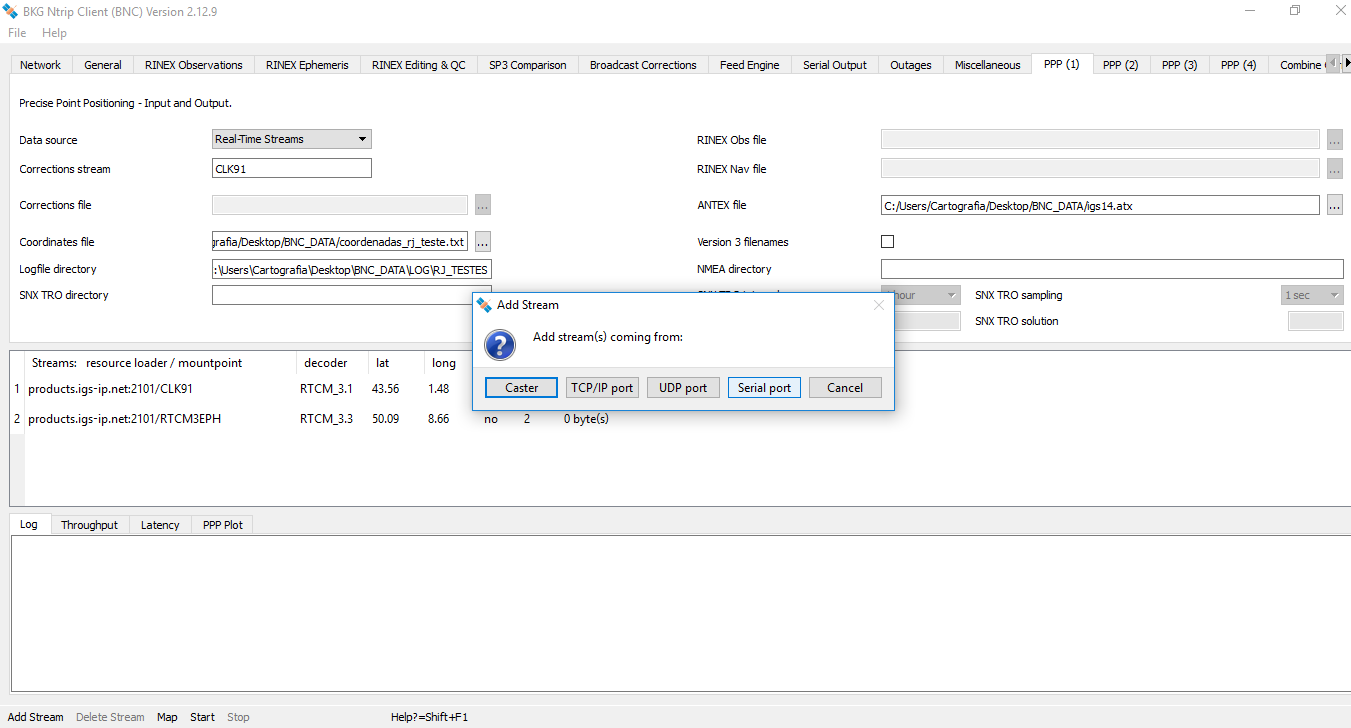
\includegraphics[scale=0.4]{img/BNC_18.png} %scale eh o tamanho que a figura vai ficar
\caption{Adição de stream \textit{stream}.}
\label{add_stream}
\end{figure}

\subsection{RTPPP com recebimento de dados do receptor via caster}
\label{rtppp_caster_bnc}
Para realizar o RTPPP dessa forma realiza-se a configuração conforme seção \ref{bnc_config} e inclui-se outro stream da seguinte forma:
\begin{itemize}
    \item \textit{Add Stream}
    \begin{itemize}
        \item \textit{Caster} - \textit{Caster host} ''\textit{www.igs-ip.net}'', porta 2101. O stream utilizado nesse trabalho foi: ''POAL00BRA0''.
    \end{itemize}
\end{itemize}



\subsection{RTPPP com recebimento de dados do receptor via porta serial}
\label{rtppp_serial_bnc}
Nesse trabalho a conexão Receptor - Computador foi feita utilizando dois cabos: Serial/COM (fêmea) e COM (Macho) - COM (Macho). O segundo cabo foi necessário pois foi um adaptador para a porta disponível no computador utilizado. Para realizar o RTPPP dessa forma realiza-se a configuração conforme seção \ref{bnc_config} e inclui-se outro \textit{stream} da seguinte forma:
\begin{itemize}
    \item \textit{Add Stream}
    \begin{itemize}
        \item \textit{Serial port} - A configuração utilizada nesse trabalho foi:
        \begin{itemize}
            \item \textit{Mountpoint} - ''RJ$_$teste'' - A denominação da \textit{Mountpoint} é de acordo com o usuário, devendo ser o mesmo dado no arquivo de coordenadas;
           \item \textit{Format} - ''RTCM$_$3'' - Formato que o BNC fará a leitura dos dados recebidos pelo receptor. É importante ressaltar que essa configuração deve estar coerente com a configuração dos dados de saída do receptor, nesse trabalho o receptor estava configurado para enviar dados no formato ''RTCM 3.x'';
            \item Latitude e Longitude - valores aproximados e inteiros, somente para exibição na lista da tela;
            \item \textit{Country} - País onde está localizado o receptor. Somente para fins de exibição em tela;
            \item \textit{Port name} - ''COM1'' - No sistema operacional Windows por padrão a porta ''COM'' é denominada ''COM1'' ou ''COM2'', vale ressaltar que no computador utilizado a cada vez que a conexão com o receptor era refeita o sistema criava um novo nome, como por exemplo ''COM6'' - Esse é o nome da porta em que o receptor está conectado via cabo.
            \item \textit{Baud rate} - 115200 - Recomenda-se que seja tão alta quanto possível.
            \item \textit{Data bits} - 8
            \item \textit{Stop bits} - 1
            \item \textit{Parity} - \textit{None}
            \item \textit{Flow control} - \textit{Off}
            \item As configurações de \textit{Baud rate}, \textit{Data bits}, \textit{Stop bits}, \textit{Parity}, \textit{Flow control} devem ser idênticas com a configuração estabelecida na saída de dados do receptor.
        \end{itemize}
    \end{itemize}
\end{itemize}

A figura \ref{bnc_stream_serial} explicita os passos explicados na seção \ref{rtppp_serial_bnc}:
\begin{figure}[H]
\centering
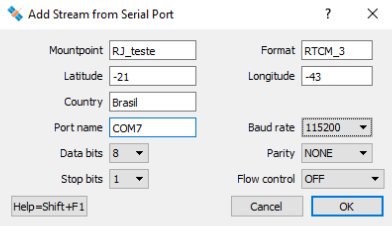
\includegraphics[scale=0.4]{img/BNC_19.png} %scale eh o tamanho que a figura vai ficar
\caption{Adição de stream via porta serial.}
\label{bnc_stream_serial}
\end{figure}

Realizadas as configurações explicadas nas seções \ref{bnc_config} e \ref{rtppp_caster_bnc} ou \ref{rtppp_serial_bnc}, aciona-se o botão \textit{start} para começar o recebimento e processamento de dados. A figura \ref{receb_dados_bnc} mostra tal recebimento.

\begin{figure}[H]
\centering
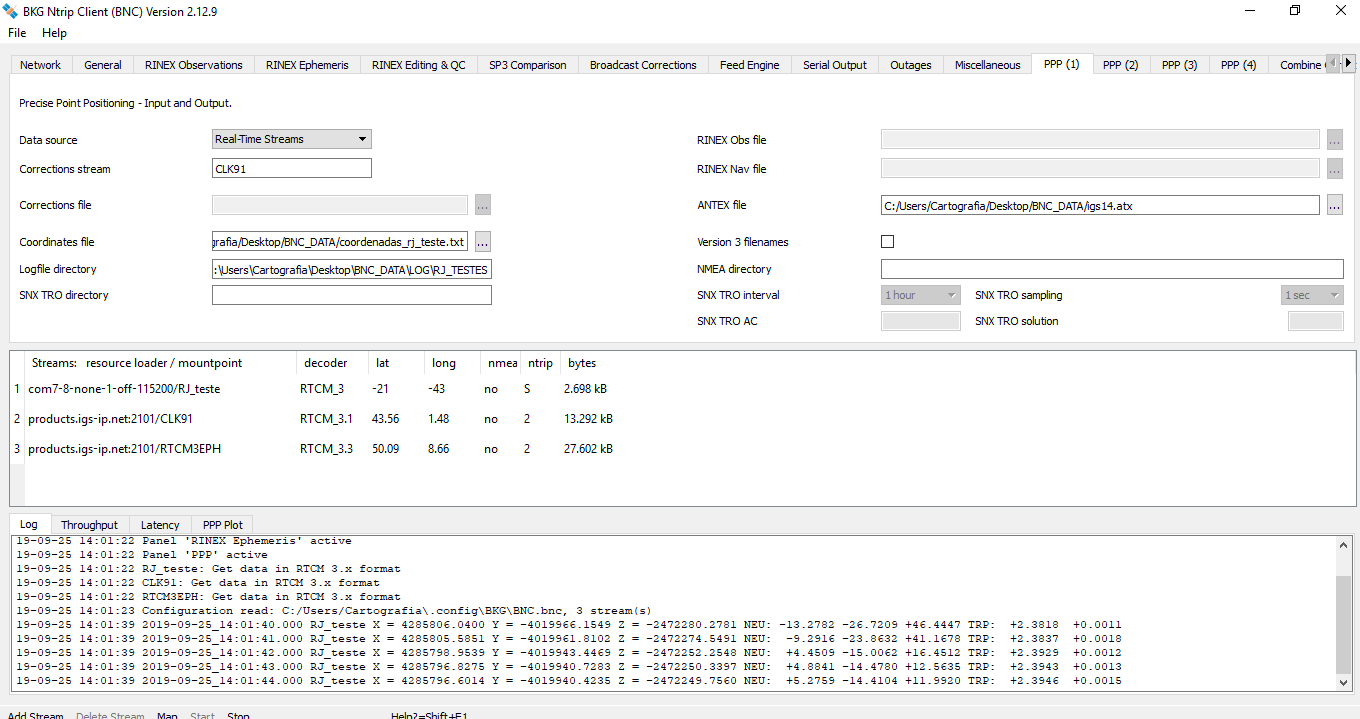
\includegraphics[scale=0.4]{img/BNC_21.png} 
\caption{Chegada de dados e processamento no BNC.}
\label{receb_dados_bnc}
\end{figure}

\section{Configuração do PPP-Wizard para realização do PPP-RTK}

Para a realização do PPP-RTK nesse trabalho utilizou-se o software PPP-Wizard, uma modificação do código do BNC que utiliza solução fixa de ambiguidades ao invés de solução \textit{float}. A seguir serão detalhados alguns passos para a configuração e utilização do PPP-Wizard.

Primeiramente deve-se abrir a pasta onde encontram-se os arquivos do programa diretamente no terminal (ou \textit{Prompt de comando}). Nessa pasta devem constar os seguintes arquivos básicos: \textit{conf\_get.txt}, \textit{conf\_process.txt} e \textit{rover.txt}.

O arquivo \textit{conf\_get.txt} especifica quais serão os \textit{streams} a serem conectados para o recebimento de dados e correções. A seguir o arquivo utilizado no presente projeto:

\lstinputlisting{PPPWizard141/conf_get.txt}

O usuário e senha devem ser obtidos através de cadastro no portal do IGS.

O arquivo \textit{conf\_process.txt} determina as opções do procedimento. É importante selecionar o modo \textit{mode\_PPP\_AR} e colocar o modelo da antena utilizada. A seguir um extrato do arquivo \textit{conf\_process.txt} utilizado:

\begin{lstlisting}
    mode_PPP_AR mode
    igs14.atx TRM115000.00
    1 1 0 AR/JumpsIndicators
    1 useGPS
    1 useGlonass
\end{lstlisting}

O \textit{rover.txt} informa o nome da estação e suas coordenadas aproximadas. A seguir o arquivo utilizado:
\lstinputlisting{PPPWizard141/rover.txt}

Após a manipulação desses três arquivos deve-se executar o seguinte comando no terminal:

\begin{lstlisting}
    ./getStream <conf_get.txt | ./processStream -conf conf_process.txt -rover rover.txt -dcb "*.DCB" > out_POAL_PPP_wizard.txt
\end{lstlisting}

O arquivo de saída \textit{out\_POAL\_PPP\_wizard.txt} armazenará todas as coordenadas e suas respectivas épocas.

\section{Configuração via \textit{software} TRU do Receptor (GR-5) para a comunicação com computador}

Esta seção explicará a configuração para a comunicação correta entre o receptor e computador, visando a utilização do \textit{software} BNC. A configuração é realizada através do \textit{software} TRU.

\begin{itemize}
    \item Conexão do receptor com \textit{software} TRU: \textit{Device > Connect}
    \item Seleciona-se a porta serial através do botão ''...'' e então pressiona-se o botão \textit{Connect}
\end{itemize}

\begin{figure}[H]
\centering
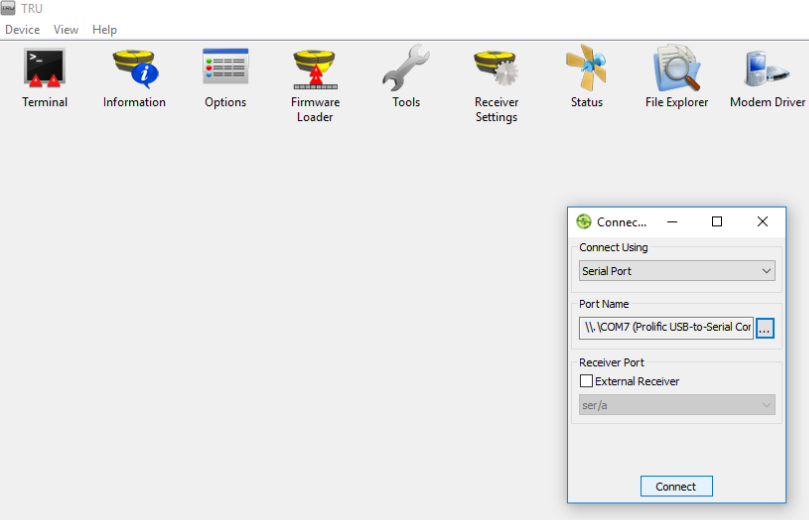
\includegraphics[scale=0.4]{pfc_pdf_files/img/TRU_3_conexao.png}
\caption{Identificação da conexão do receptor via porta serial.}
\label{Rotulo}
\end{figure}

Para a realização de qualquer levantamento RTK deve-se manter atualizado os drivers de comunicação rádio do receptor. Para tal deve-se acessar \textit{Modem Driver} > \textit{Topcon Digital UHF II Motorola H24} > \textit{Modem Properties} conforme figura \ref{conf_modem_tru}.

\begin{figure}[H]
\centering
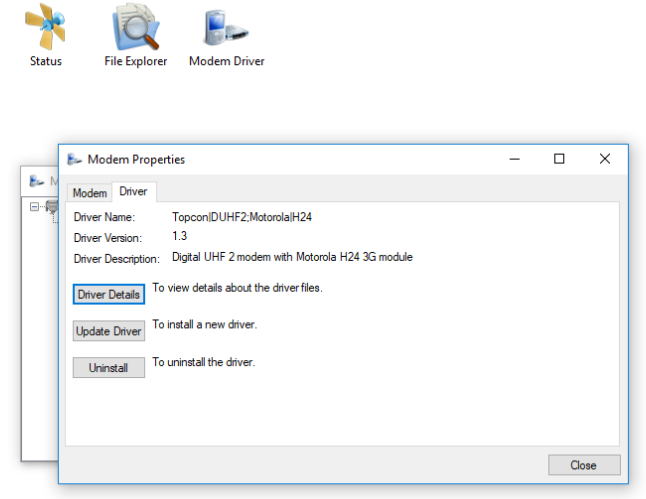
\includegraphics[scale=0.4]{pfc_pdf_files/img/TRU_5_modem.png}
\caption{Configurações de drivers.}
\label{conf_modem_tru}
\end{figure}

Para realizar as configuração das informações de entrada e saída nas portas do receptor deve-se acessar a opção \textit{Receiver Settings} conforme figura \ref{TRU_rec_settings} e em seguida acessar a opção \textit{Ports} conforme figura \ref{TRU_rec_ports}.

\begin{figure}[H]
\centering
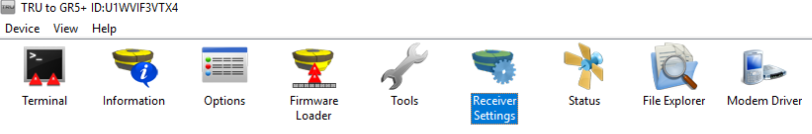
\includegraphics[scale=0.5]{pfc_pdf_files/img/TRU_6_rec_set.png}
\caption{Configurações do receptor.}
\label{TRU_rec_settings}
\end{figure}

\begin{figure}[H]
\centering
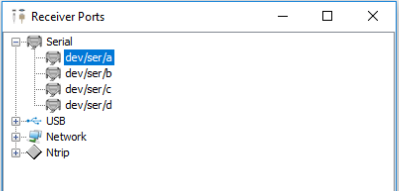
\includegraphics[scale=0.6]{pfc_pdf_files/img/TRU_7_rec_ports.png}
\caption{Configurações das portas do receptor.}
\label{TRU_rec_ports}
\end{figure}

A porta que realiza a comunicação de dados com o BNC nesse trabalho foi a porta ''dev/ser/a''. Abre-se a configuração dessa porta e seleciona-se o \textit{Output mode} para ''RTK RTCM 3.x'' na aba \textit{General}, conforme figura \ref{porta_a}.

\begin{figure}[H]
\centering
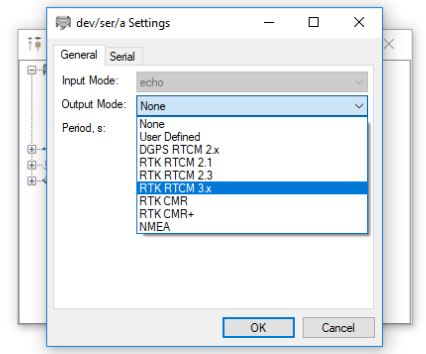
\includegraphics[scale=0.6]{pfc_pdf_files/img/TRU_9_porta_a.png} %scale eh o tamanho que a figura vai ficar
\caption{Formato dos dados de saída.}
\label{porta_a}
\end{figure}

Nessa mesma aba pode-se realizar a verificação das mensagens RTCM que o aparelho está transferindo, conforme figura \ref{msg_receptor}. Por padrão do receptor as mensagens relacionadas as efemérides do sistema GPS e GLONASS (1019 e 1020 respectivamente) não estão incluídas na configuração. Caso ao realizar o RTPPP com o BNC não se conecte ao \textit{stream} \textit{RTCM3EPH} deve-se incluir essas mensagens no aparelho, conforme figura \ref{new_msg_receptor}. Recomenda-se que se conecte ao referido caster utilizando as efemérides recebidas através dele. Ao utilizar as efemérides recebidas pelo próprio receptor nesse trabalho a seguinte mensagem de erro no BNC era transmitida: "\textit{Wrong observation epoch(s)}"

\begin{figure}[H]
\centering
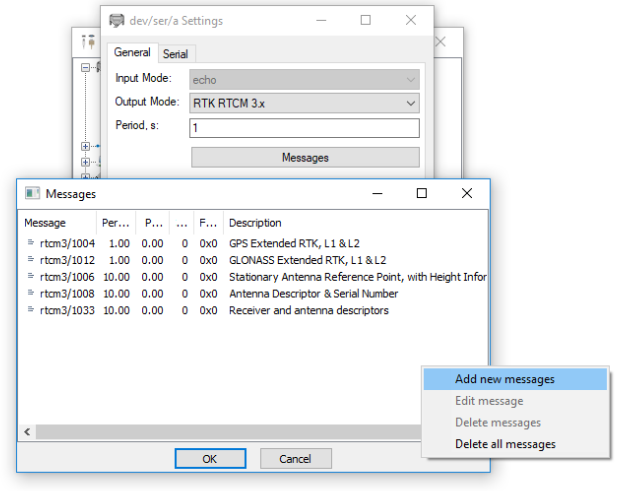
\includegraphics[scale=0.5]{pfc_pdf_files/img/TRU_13_msg.png} %scale eh o tamanho que a figura vai ficar
\caption{Verifica das mensagens transmitidas pelo receptor.}
\label{msg_receptor}
\end{figure}

\begin{figure}[H]
\centering
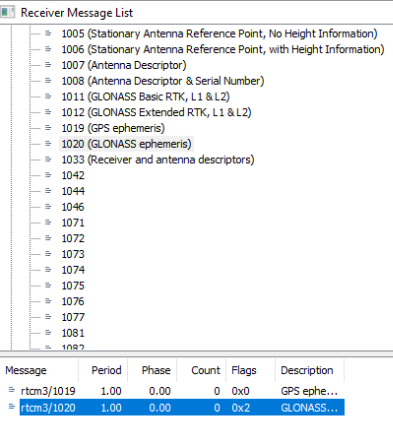
\includegraphics[scale=0.5]{pfc_pdf_files/img/TRU_14_msg.png} %scale eh o tamanho que a figura vai ficar
\caption{Inclusão de novas mensagens para a transmissão.}
\label{new_msg_receptor}
\end{figure}


Na aba \textit{Serial} da mesma janela são realizadas as configurações da transmissão de dados da porta serial. Tais dados devem ser configurados de forma idêntica aos configurados no BNC conforme explicado na seção \ref{rtppp_serial_bnc} e figura \ref{TRU_serial}.

\begin{figure}[H]
\centering
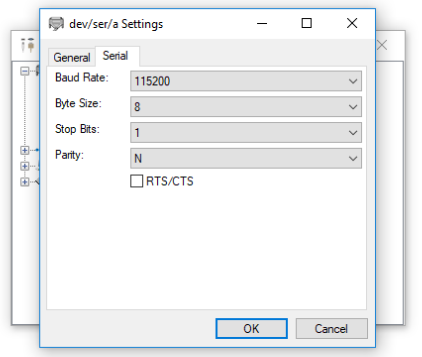
\includegraphics[scale=0.4]{pfc_pdf_files/img/TRU_11_porta_a.png} %scale eh o tamanho que a figura vai ficar
\caption{Configuração de Baud Rate, Byte Size, Stop Bits e Parity.}
\label{TRU_serial}
\end{figure}

O receptor GR-5 armazena os dados do levantamento em cartão de memória SD, nesse trabalho não foi possível acessar os dados gravados diretamente no cartão, para tal foi necessário acessar os dados através do TRU conforme figura \ref{TRU_dados}.

\begin{figure}[H]
\centering
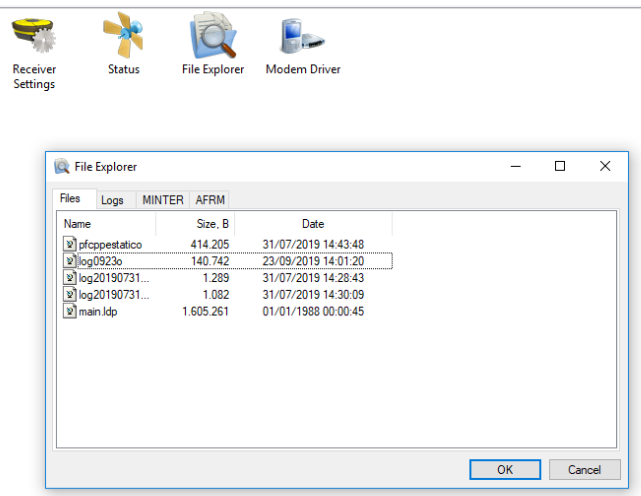
\includegraphics[scale=0.4]{pfc_pdf_files/img/TRU_17_dados.png} %scale eh o tamanho que a figura vai ficar
\caption{Visualização dos arquivos gravados no receptor.}
\label{TRU_dados}
\end{figure}

\section{Configuração do receptor via controladora para realização de RTK}

A fim de realizar as configurações necessárias para a realização de RTK com o receptor GR-5 é interessante a utilização da controladora devido sua portabilidade. A seguir serão descritas algumas configurações básicas a a realização desse método com o GR-5. Cabe ressaltar que caso a comunicação via \textit{bluetooth} entre o receptor e a controladora não esteja funcionando deve-se conectar o receptor ao TRU e alterar a taxa de transmissão da porta "/dev/serial/d'' para 115200.

Após a conexão do receptor com a controladora deve-se abrir a janela ''Configuração'', nomear a configuração e escolher o tipo de método, conforme figura \ref{controladora_conf}.

\begin{figure}[H]
\centering
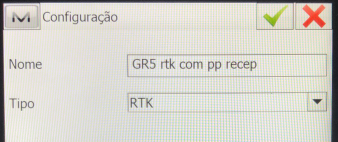
\includegraphics[scale=0.5]{pfc_pdf_files/img/controladora_conf.png} %scale eh o tamanho que a figura vai ficar
\caption{Tela de início para configuração de RTK.}
\label{controladora_conf}
\end{figure}

Escolhe-se o valor para máscara de elevação e o formato para as correções diferenciais enviadas do receptor base para o receptor rover, conforme figura \ref{controladora_cor}

\begin{figure}[H]
\centering
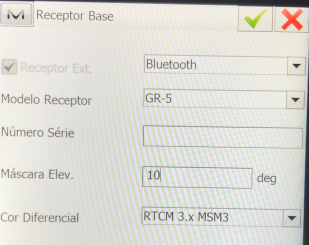
\includegraphics[scale=0.5]{pfc_pdf_files/img/controladora_2.png} %scale eh o tamanho que a figura vai ficar
\caption{Tela correções RTK.}
\label{controladora_cor}
\end{figure}

Escolhe-se onde será feito o armazenamento dos dados, se na controladora ou no receptor conforme figura \ref{controladora_arq}. Recomenda-se que tanto para a Base quanto para o Rover selecione-se "Receptor" visto que nas tentativas realizadas nesse trabalho para arquivamento na controladora os dados não foram armazenados.

\begin{figure}[H]
\centering
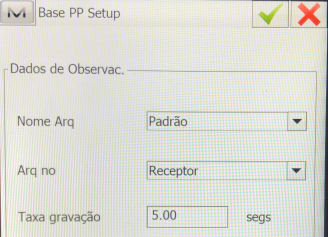
\includegraphics[scale=0.5]{pfc_pdf_files/img/controladora_arq.png} %scale eh o tamanho que a figura vai ficar
\caption{Tela de início para configuração de RTK}.
\label{controladora_arq}
\end{figure}

Escolhem-se as configurações de rádio, conforme figuras \ref{controladora_radio} e \ref{controladora_radio2}.

\begin{figure}[H]
\centering
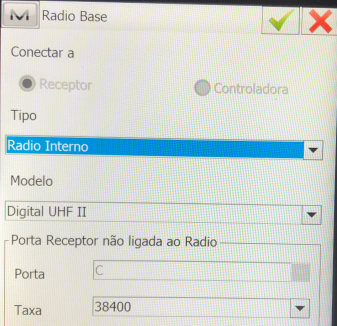
\includegraphics[scale=0.5]{pfc_pdf_files/img/controladora_radio.png} %scale eh o tamanho que a figura vai ficar
\caption{Tela configuração de rádio RTK.}
\label{controladora_radio}
\end{figure}

\begin{figure}[H]
\centering
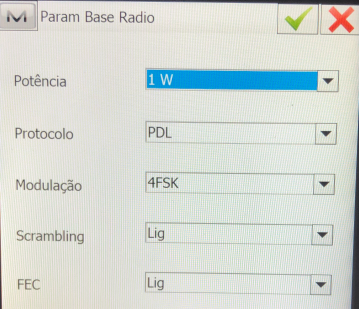
\includegraphics[scale=0.4]{pfc_pdf_files/img/controladora_radio2.png} %scale eh o tamanho que a figura vai ficar
\caption{Tela 2 configuração de rádio RTK.}
\label{controladora_radio2}
\end{figure}

Realizadas essas configurações as telas se repetirão para determinar as configurações do \textit{rover} que são idênticas a configuração do \texti{base}. As demais telas de configuração são intuitivas.

Após a realização das configurações deve-se iniciar o receptor base, conectar ao receptor rover e então coletar os pontos desejados. 

Cabe ressaltar que para iniciar o receptor base deve-se inserir as coordenadas do ponto em que ele está posicionado ou solicitar que as coordenadas obtidas via GNSS sejam utilizadas. Caso se escolha por inserir as coordenadas manualmente recomenda-se a utilização de coordenadas geográficas visto que nesse trabalho ao utilizar-se de coordenadas cartesianas o sistema trocava as coordenadas X e Y e exibia a mensagem de erro que o receptor estava a mais de 500 metros do ponto informado.




